\subsection{Pipeline}

Our pipeline will consist of the stages that can be seen in figure \ref{fig:pipeline}. First of all data from two different sources will be downloaded, temporarily stored and cleaned up to disregard records with missing data.
All cleaned up records will be stored permanently so we don't have to download and clean up the data every time we change some downstream settings. From this data storage the text we are going to use in the end will be extracted and some clustering algorithms will be used to build the final result.

\begin{figure}[ht]
    \centering
    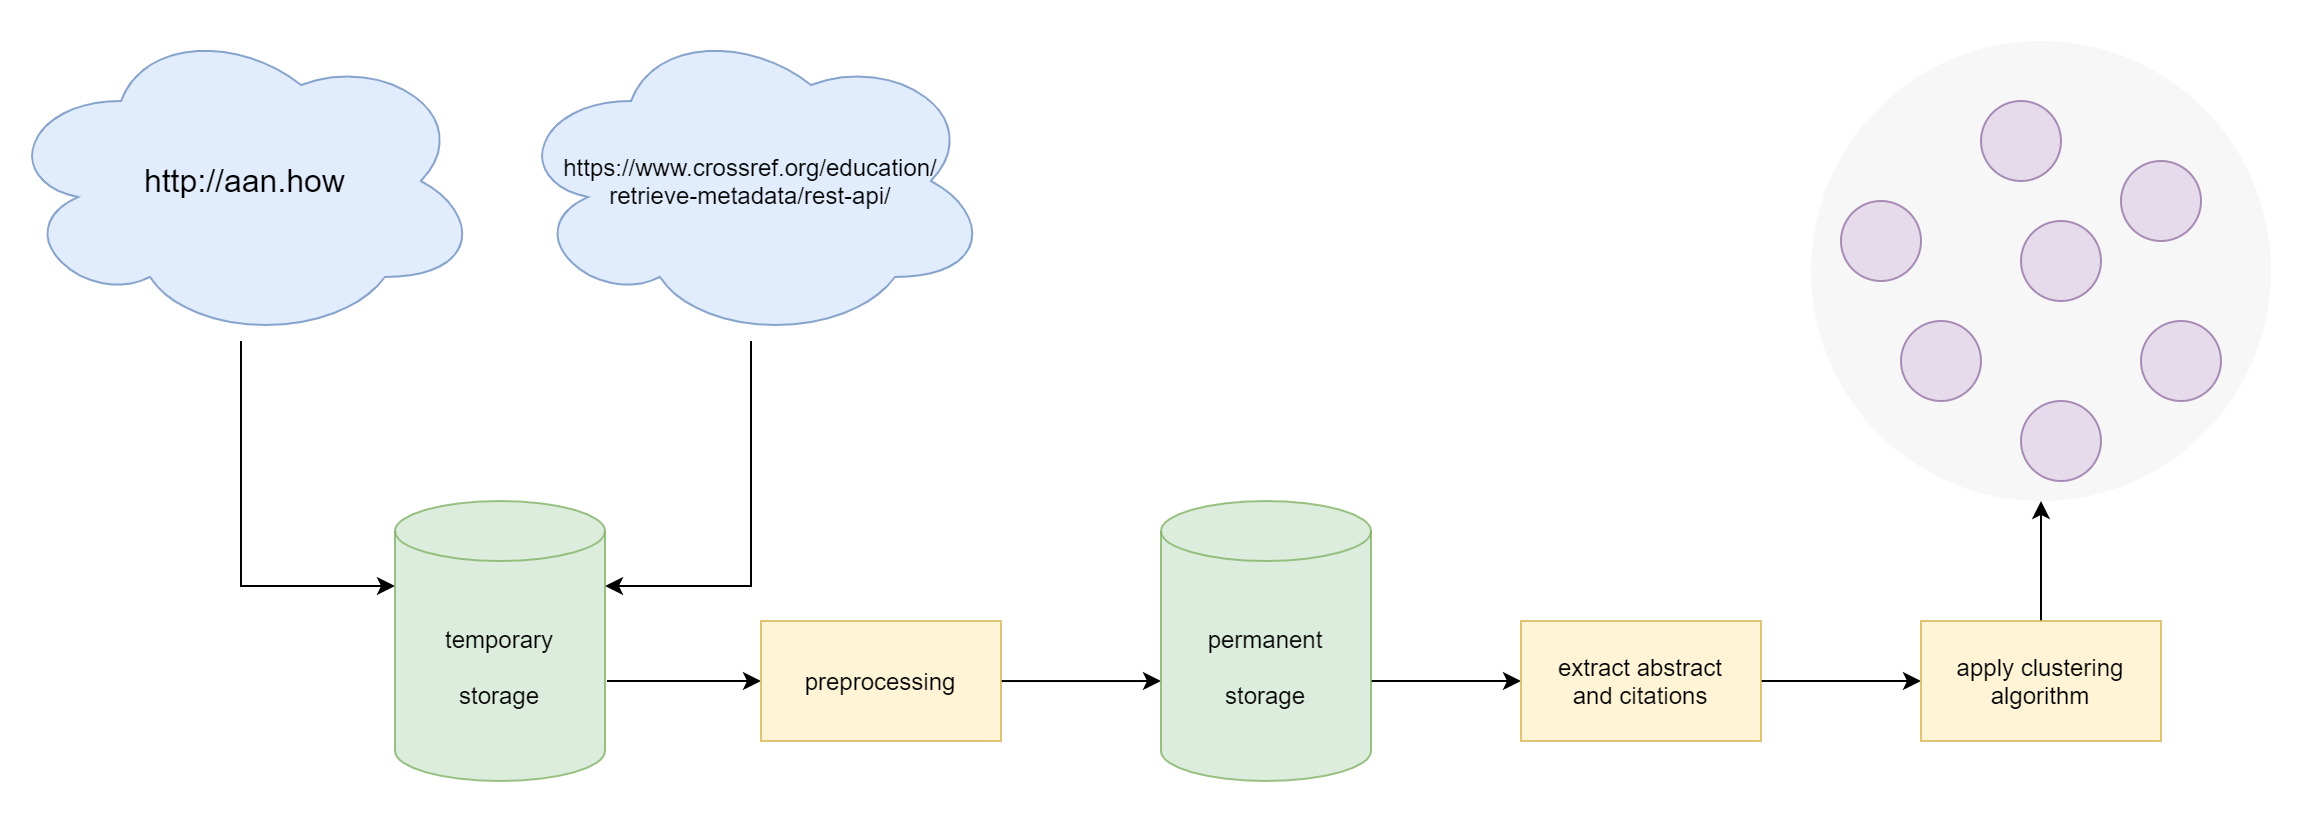
\includegraphics[width=\textwidth,keepaspectratio]{figures/pipeline}
    \caption[]{Coarse overview over the intended pipeline.}
    \label{fig:pipeline}
\end{figure}

